\documentclass[msc,oneside]{ubcthesis}%msc, phd, masc, ma, or meng

% ================================================================================
% CHANGE THE FOLLOWING ACCORDING TO YOUR PROGRAM/THESIS
% ================================================================================
\institution{The University Of British Columbia}
\program{Computer Science}
\faculty{THE IRVING K. BARBER SCHOOL OF ARTS AND SCIENCES}
\institutionaddress{Okanagan}

% For an Honours thesis, use \documentclasss[msc,oneside]{ubcthesis} above and
% uncomment and modify the next line:
\degreetitle{B.Sc. Computer Science Honours}

\title{The Source}
%\subtitle{With a Subtitle}
\author{Raffi Kudlac} % The name needs to be exactly the same as on the diploma i.e. (Name from SISC)
\copyrightyear{2015}
\submitdate{April 2015} % date of approved thesis
%\program{Interdisciplinary Studies - Optimization}%or Mathematics, or Interdisciplinary Studies
%\previousdegree{B.Sc. Hons., The University of British Columbia, 2008}
%\previousdegree{M.Sc., The University of British Columbia, 2010}

% ================================================================================


\usepackage{ubcostyle} %loads packages


% ===================================================================
% CHANGE THE FOLLOWING COMMANDS ACCORDING TO YOUR NEEDS
% ===================================================================
\newcommand{\R}{\mathbb{R}}   %real number
\newcommand{\Z}{\mathbb{Z}}   %integers
\newcommand{\C}{\mathbb{C}}   %complex numbers

\newcommand{\dom}{\operatorname{dom}}
\providecommand{\TT}[1]{\Theta\left(#1\right)} % big-Theta
\providecommand{\OO}[1]{\mathcal{O}\left(#1\right)} % big-Oh
% ===================================================================

%Uncomment the next line if there are more than one appendix
%\renewcommand*\appendixname{Appendices}


\begin{document}

% This starts numbering in Roman numerals as required for the thesis
% style.
\frontmatter                    % Mandatory

% The order of the following components should be preserved.  The order
% listed here is the order currently required by FoGS.
\maketitle                      % Mandatory

\newpage
\phantomsection \label{tableofcontent}%set anchor at right location
\addcontentsline{toc}{chapter}{\contentsname}
\tableofcontents                % Mandatory: generate toc
\newpage 
\phantomsection \label{listoftab}%set anchor at right location
\addcontentsline{toc}{chapter}{\listtablename}
\listoftables                   % Mandatory if thesis has tables
\newpage
\phantomsection \label{listoffig}%set anchor at right location
\addcontentsline{toc}{chapter}{\listfigurename}
\listoffigures                  % Mandatory if thesis has figures

% Any other unusual prefactory material should come here before the
% main body.

% Now regular page numbering begins.
\mainmatter

% Parts are the largest structural units, but are optional.
%\part{Thesis}

% Chapters are the next main unit.
\chapter{Introduction}
	“The Source” is an interactive simulation model where the user is charged with the task of providing 
energy to a growing population. The purpose of the simulation is to show the benefits and detriments of 
each type of energy source. Although the game targets young adults, primarily around high school and 
College/university students; anyone can play and and have a learning experience. Two intended outcomes of 
the simulation are to demonstrate the ratio of energy output to energy source type, and show the inner 
workings of each. A third outcome of the simulation is show that each type of energy works in the same way 
at its most basic level, with the exception of solar power converting kinetic energy into electrical energy.
\bigskip

The user will accomplish the task of providing energy by choosing to invest in different types of energy. 
The energy types that are at the users' disposal are solar, wind, hydro, coal, oil, gas and nuclear. Users 
can choose to build any of these power plants, but each type has consequences that others may not have. For 
example, if a user decided to build a power plant that ran off of coal, environmentalists would be 
displeased because the burning of coal introduces pollutants into the atmosphere. As well as considering 
the consequences of their actions, the users must also consider what fuels each power plant and how long 
each power plant can be sustained for. Fossil fuels and nuclear power are not infinite; the user must find 
resources to fuel these power plants. Users can choose to invest in renewable resources such as solar, wind 
and hydro, but the problem the user encounters with these types of resources is that they don't output as 
much energy as fossil fuels. The users' main objective is to survive for as long as possible and to beat 
their previous time. 

\chapter{Energy Today}
	In our society today almost all electrical energy is converted in the same way, converting kinetic 	
to moving this magnet. In almost all designs the magnet is connected to a turbine,which can be rotated, so 
that if the turbine obtains kinetic energy it can be transferred to the magnet. How the turbine acquires 
kinetic energy is different depending on the sours of energy. In the case of Fossil fuels and nuclear 
power, all that is happening is that water is being turned into steam and then the steam is used like wind 
to turn the turbine to make power. In the case of hydro power, the flowing water turns the turbine and in 
the case of wind power the turbine is physically connected to the rotating blades throughout the shaft of 
the windmill. 
\bigskip

The exception, solar power. Solar Power works a little different, the general idea is that when beamsof 
light hit the solar panels some of the energy from the light doesn’t get transferred into heat and is 
instead transferred into the electrons. With their newly obtained energy the electrons become free and able 
to move around. This makes a current possible and from here it is just a matter of extracting it.
\bigskip

It could be argued that nuclear power plants, fossil fuel plants and big hydro dams are these big complex 
systems that generate our power for us but they all work off the one basic idea of moving a magnet through 
a copper coil. This centuries old idea has fundamentally redirected the evolutionary direction of our 
society today. 


\chapter{The Sourse}

The design of the system, as illustrated in figure 3.1 below, is straightforward. The user interacts with 
the system by purchasing power plants. This is done on a designated screen when there is land for the user 
to build on. Once the user has picked a type of power he/she must then provide the resources necessary for 
the power plant to function. The user can obtain fossil fuels by mining for them on the screen designated 
to represent the land that is currently available for the user to excavate. Once resources have been 
obtained and a power plant is built, energy can then be created and supplied to the population.
\bigskip

Another option that the user has is that he/she can purchase advertisements or public services to help 
him/her flourish in the simulation. For example, a user could purchase an advertisement that educates the 
population to not waste power. This advertisement would reduce the usage of power and allow the user to 
more easily meet the demand. Users can also buy public services. An example would be a geologist that would 
survey the land and tell the user where to mine for a specific resource. Both of these purchases can 
influence groups within the game, such as environmentalists or public opinion. 
\bigskip

Users choices in the game affect groups as well, for example if a user invested in coal fueled power plants then the environmentalists group would not be displeased. Groups provide small perks or punishments to the user, usually in the form of grants or fines, which are dependent on the users play style and choices within the simulation. 

\begin{figure}[ht]
  \begin{center}
    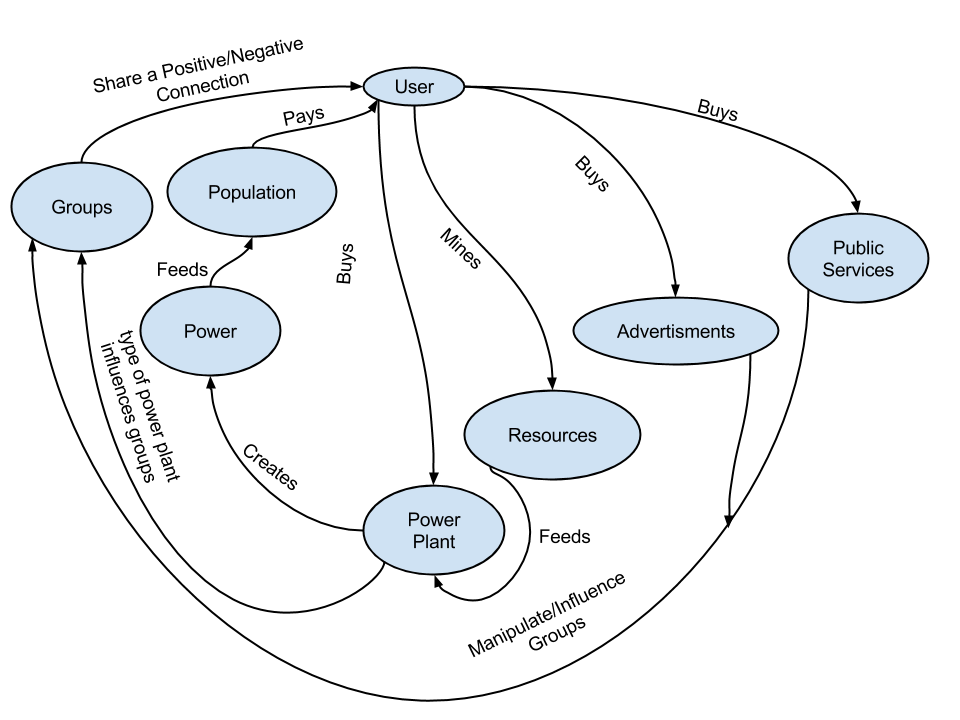
\includegraphics[width=1\textwidth]{DFDDiagram}
    \caption[Figure 1]{\label{DFD Diagram} }
  \end{center}
\end{figure}


\section{Screen Layout}
“The Source” is composed of 8 different screen. The first five mentioned below are know as the five core screens. You can get to any of these screens from any other screen in the game. 
\bigskip

\noindent \large \textbf{ The Business Screen (one of the five core screens):} \newline
\indent In this screen the user is able to purchase advertisements and pubic services to help him/her 
progress through the simulation. Here the user is also able to see their progress throughout the game. The 
user will be able to see data like, money and energy made over time.  
\bigskip

\noindent The City Screen (one of the five core screens): \newline
\indent Here the user is able to see how the population is doing, the amount of power currently demanded and the amount supplied. This screens purpose is to purely display information.
\bigskip

\noindent The Power Plant Screen (one of the five core screens): \newline
\indent This screen, possibly the most education screen shows the workings of each type of energy as well as the inner workings of a generator. As well as seeing this information this screen allows the user to 
see specifics on the current power plants that he/she has built. Specifics being information such as 
amount of power produced, cost to maintain, resources required to maintain and more. 
\bigskip

\noindent The Land Screen (one of the five core screens): \newline
\indent From this screen the user can build power power plants that run off of fossil fuels and uranium. The user will have some designated land to start but he/she also has the option to buy more land to build 
on if the starting land is all used up.
\bigskip

\noindent The Resource Screen (one of the five core screens): \newline
\indent The purpose of this screen is to act like a map for the resources at the users disposal. From this 
screen the user can see all the resource that will be needed and the user can get at the three resource 
screens that will allow the user to extract the resources.
\bigskip

\noindent The Hydro Screen: \newline
\indent From here the user can view numerous rives that could be damned in order to generate power. Once a 
river is damned it will be shown on the screen. Rivers can only be damed once. 
\bigskip

\noindent Solar/wind Power Screen: \newline
\indent This screen shows land in the form of a grid that the user has at his/her to build windmills on or 
solar canals. Building will have a cost. Once something is built it can be dismantled to open the land 
to have something else built. 
\bigskip


\noindent The Fossil Fuels Screen: \newline
\indent Here land that the user can mine will be shown. This will be one large grid that will hold all the 
fossil fuels and uranium. The user can mine a section by selecting it and he or she will have a chance 
of discovering any one of the four resources. The resource discovered will go towards fueling the built 
power plants. Once a section is mined it can not be reused. 
\bigskip

\noindent The Static Screen: \newline
\indent The static screen is not really a screen at all but a combination of static images that remain on 
top of all other screens for the entire duration of the game. This serves as the means of navigation 	
between the five core screens. As well as displaying some information such as money and time. 
\bigskip

%Include citations in your thesis as you write:
%\cite{MR2848848,MR2461448,MR2834159,infconv,convmono,MR2668638,Bauschke:2007-PA02,proxbas}

%\section{Packages}
%There are several packages\ . So before you add a new package, check first if it is already included there.


%\section{Epigraph}
%If you want to add an epigraph to a chapter (epigraph in the sense of a literary inscription, not a function epigraph), you can use the command \texttt{epigraph} after the chapter. Check out the documentation of the \texttt{epigraph} package for more information.

% The following are examples of how to incorporate graphics into your thesis.

% \begin{figure}[ht]
%   \begin{center}
%     \includegraphics[width=0.4\textwidth]{figure}
%     \caption[Sample figure.]{\label{fig:happy} This is a sample figure
%       Note that we have
%       used the optional argument for the caption command so that only
%       a short version of this caption occurs in the list of figures.}
%   \end{center}
% \end{figure}

% \begin{figure}[ht]
%   \begin{center}
%     \includegraphics[width=0.4\textwidth]{figure}
%     \caption{\label{fig:happy2} This is the same sample figure with still
% 			a long caption but this time we did not use a short caption command
% 			in the table of figures.}
%   \end{center}
% \end{figure}

% You should really put text in between figures so LaTeX has more flexibility to place the figure at the appropriate location.



\chapter{Sample Content Using Mathematical Notations}

\section{Facts and theorems}
If we use a well established fact or theorem\ 

\begin{fact}\cite[Theorem~IV.2.4.2]{Hiriart-Urruty:1993-ConvexAnalysis}\label{def:marginalfunc}
Define the \emph{marginal function} $\gamma$ associated with $g:\R^n\times\R^m\rightarrow \R\cup
\{+\infty\}$ by $z\mapsto \gamma(z):=\inf_x
g(x,z)$. If $g$ is a proper convex function and is bounded below on the set  $\R^n \times \{z\}$ for all $z$, then $\gamma$ is convex.
\end{fact}

\section{Propositions and lemmas}
Here is a lemma followed by its proof.
\[
D =\left\{ (x,\lambda)\in \R^d \times \R^+ : \frac{x}{\lambda} \in C\right\}.
\]

\begin{lemma}
Assume $C$ is a nonempty closed convex set. Then the set $D$ is a nonempty closed convex cone.
\end{lemma}

\begin{proof}
The fact that $D$ is nonempty and closed follows from $C$ being non\-empty and closed. One can check directly that $D$ is a cone....

Hence $D$ is convex.
\end{proof}
Make sure that the qed symbol is always on the last line of the proof. If the last line is an equation, you can enforce the qed on the same line with the \texttt{qedhere} command.

For citations, please use BibTex. A sample article to verify formatting and style is \cite{Bauschke:2007-PA02}. Use the bibliography style \texttt{ubco}, which is basic \texttt{alphaurl} style with inline links enabled. Please compile multiple times when generating the references. The last entry in a reference are the back references to the pages with the citation. They need an additional compilation, once the bibtex entries are generated.

Note that the bibliography style is discipline dependent so feel free to use the style adopted by your discipline, for example siam for mathematics.

\chapter{Landscape Mode}
The landscape mode allows you to rotate a page through 90 degrees.  It
is generally not a good idea to make the chapter heading landscape,
but it can be useful for long tables etc.

\begin{landscape}
  This text should appear rotated, allowing for formatting of very
  wide tables etc.  Note that this might only work after you convert
  the \texttt{dvi} file to a postscript (\texttt{ps}) or \texttt{pdf}
  file using \texttt{dvips} or \texttt{dvipdf} etc.
\end{landscape}

\chapter{Conclusion}
Here comes the conclusion.
\begin{table}[tbph]
\centering
\caption{A publication quality table. Very very very very very very very very very very long title.
\label{table:food1}}
\begin{tabular}{@{}llr@{}} \toprule 
\multicolumn{2}{c}{Item} \\ \cmidrule(r){1-2} 
Animal & Description & Price (\$)\\ \midrule 
Gnat & per gram & 13.65 \\ 
& each & 0.01 \\ 
Gnu & stuffed & 92.50 \\ 
Emu & stuffed & 33.33 \\ 
Armadillo & frozen & 8.99 \\ \bottomrule 
\end{tabular}
\end{table}

\newpage
Your conclusion can go on for several pages.


% This file is setup to use a bibtex file sample.bib and uses the
% plain style.  Other styles may be used depending on the conventions
% of your field of study.
%
% Note: the bibliography must come before the appendices.


%change heading ``Chapter 5 Bibliography''->''Bibliography''
\newpage %newpage needed otherwise pagestyle applied to previous chapter. Does not actually create a new page
\pagestyle{fancy}\chead{Bibliography}\rhead{}\cfoot{}\rfoot{\thepage}

%Bibliography style is discipline dependent. Mathematic student can use e.g. SIAM
\bibliographystyle{ubco}
%\bibliographystyle{siam}
\bibliography{bibliography}%name of your .bib file

\newpage
\pagestyle{headings}
\addtocontents{toc}{%
\protect\renewcommand*\protect\cftchappresnum{\appendixname~}}

\appendix 
\addappheadtotoc %uses the current page number when it makes the entry in the ToC
\appendixpage 

\addtocontents{toc}{
\setlength{\cftbeforechapskip}{\cftbeforesecskip}
\setlength{\cftchapindent}{\cftsecindent}
\protect\renewcommand{\cftchapfont}{\cftsecfont}
\protect\renewcommand{\protect\cftchapdotsep}{\cftsecdotsep}
}


\chapter{Tables}
Here you can have additional tables. Table captions are always on top.

In order to use publication quality tables, one should use the guidelines in \cite{Fear:2005manual}. In short, do not use vertical rules or double rules, units in the column heading (not in the body of the table), precede decimals with a digit, and do not use ditto signs. Table \ref{table:food} is according to the guidelines. 

For tables, the caption goes on top, for figures, the caption goes on the bottom. If possible, always position tables and figures at the top of a page.\footnote{In this case, the chapter heading prevents the table from being at the top.} Use the option \verb|tbph| for the placement.

\begin{table}[tbph]
\centering
\caption{A publication quality table. Very very very very very very very very very very long title.
\label{table:food}}
\begin{tabular}{@{}llr@{}} \toprule 
\multicolumn{2}{c}{Item} \\ \cmidrule(r){1-2} 
Animal & Description & Price (\$)\\ \midrule 
Gnat & per gram & 13.65 \\ 
& each & 0.01 \\ 
Gnu & stuffed & 92.50 \\ 
Emu & stuffed & 33.33 \\ 
Armadillo & frozen & 8.99 \\ \bottomrule 
\end{tabular}
\end{table}

\newpage
And other table materials (I needed to generate two pages for that appendix to test the formatting of the table of content).

\begin{table}
\caption{Another table}
\end{table}

\begin{table}
\caption{Another table}
\end{table}
\begin{table}
\caption{Another table}
\end{table}
\begin{table}
\caption{Another table}
\end{table}
\begin{table}
\caption{Another table}
\end{table}

\begin{table}
\caption{Another table}
\end{table}
\begin{table}
\caption{Another table}
\end{table}
\begin{table}
\caption{Another table}
\end{table}
\begin{table}
\caption{Another table}
\end{table}
\begin{table}
\caption{Another table}
\end{table}

\chapter{Figures}
Here you can have additional figures. Figure captions are always at the bottom.

\newpage

And other additional figures (again I needed to generate two pages :-).
% Indices come here.


\end{document}
\endinput
